\section{Project Introduction}
\subsection{Overview of the Problem}
Standard electric meters were developed decades ago and are still used today, despite many technological advances in the last several years. Along with these technological advances, Americans have become accustomed to having access to large amounts of data, but due to the nature of the standard electric meter, data regarding the usage of power is severely limited. For the power companies, data from the meters is minimal and grid control is limited to manual operation, costing them time and money.
As the cost of electricity becomes higher and higher, electricity use in buildings is becoming a bigger concern and people have few cheap or simple ways to monitor this. Of the options available, most only address part of the whole problem, giving some information to the consumer and none to the power company or vice-versa. While there are devices such as breakers and fuses that provide electrical safety for buildings, advances in technology have made it possible to further improve safety but have not been implemented in a cost-effective way or made easily available to an average consumer, which for the purpose of this project shall be defined as a person without a mathematical or scientific education beyond high-school.

\subsection{Why the Project was Chosen}
Our team chose the project for several reasons; as future homeowners, the team has an interest in knowing more about power usage within a home. There are also many more people who would benefit from more accurate and useful data about power usage.

As good stewards of Earth we want to make sure the natural resources available are not wasted, and we believe that if there is access to more and better information, people will have a better opportunity to manage those resources more effectively. In addition, providing better information and control to the power companies can lead to less wasting of electricity on the provider's end, further contributing towards better use of Earth's resources.

Electricity-related deaths and injuries have been reduced due to devices such as fuses and breakers, but many still happen every year. As fellow human beings, we care and would like to minimize these incidents further. The technology is available and will benefit many people when implemented.

\subsection{Team Information}

Team 01, Team PICA seen in figure \ref{fig:teamphoto} consists of four engineers in Calvin College's Electrical and Computer Engineering concentration: Amy Ball, Nathan Jen, Avery Sterk, and Kendrick Wiersma.

\begin{figure}[htbp]
\begin{center}
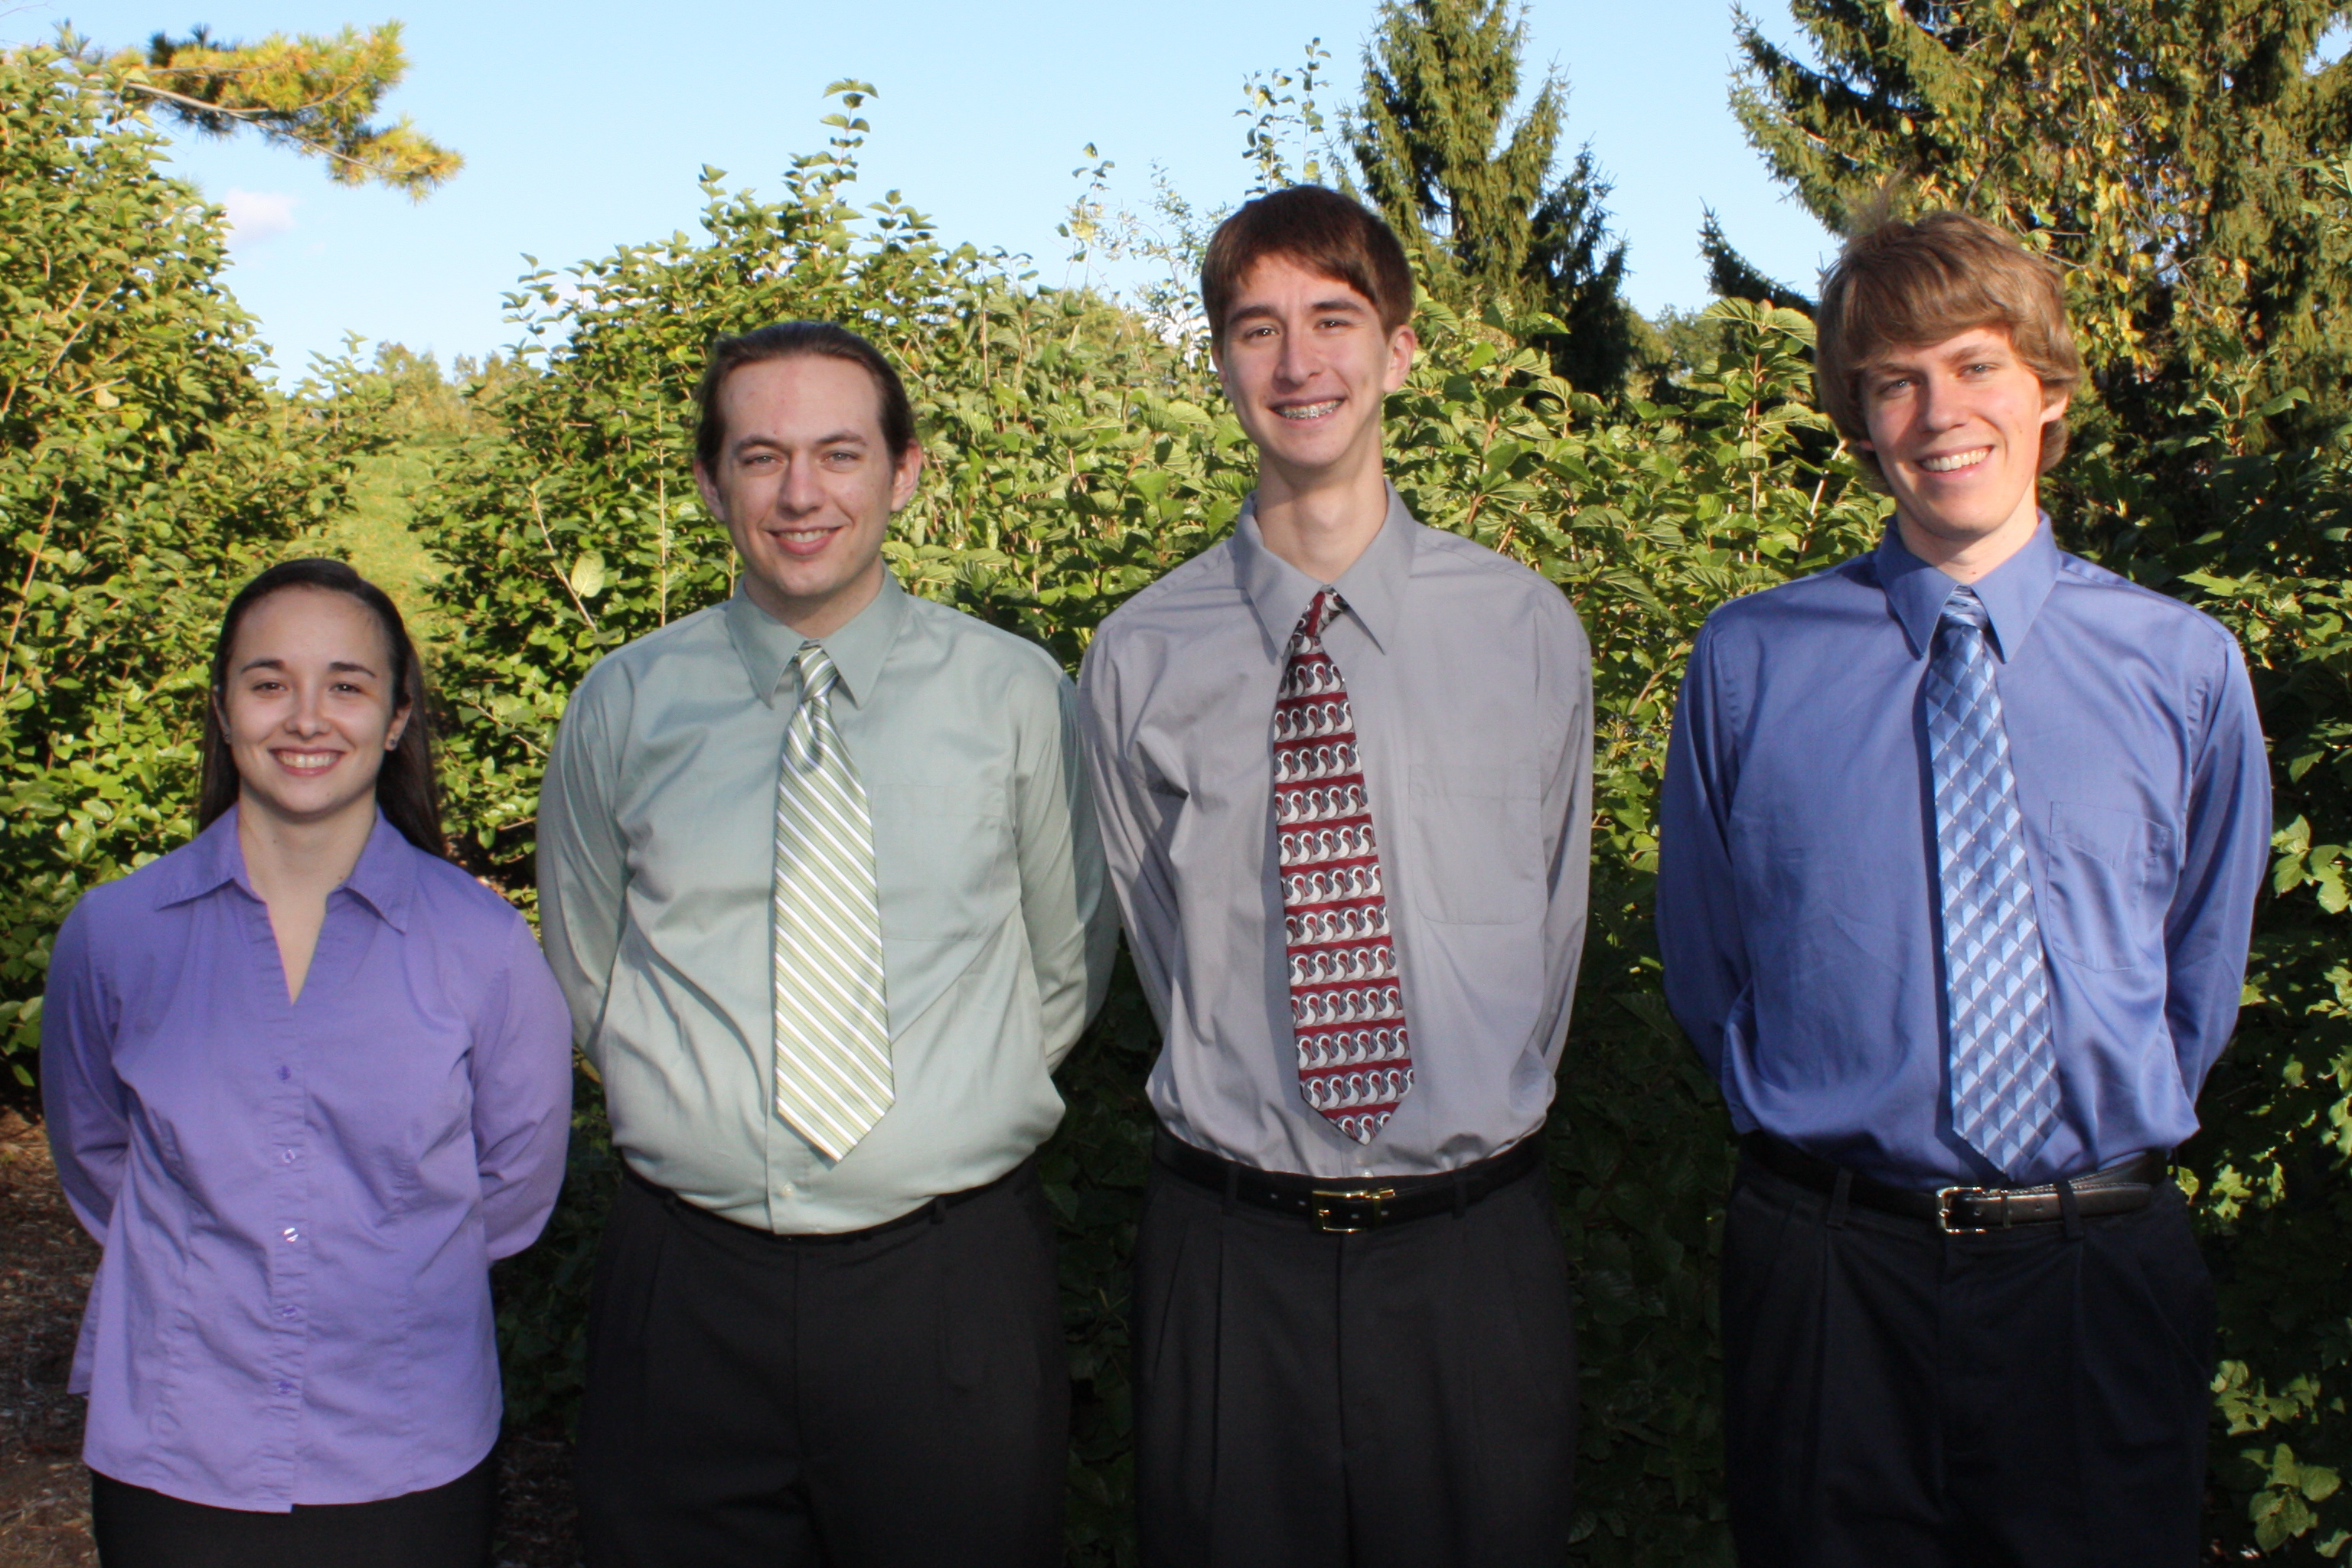
\includegraphics[width=6in]{figures/IMG_0865}
\caption{Team PICA, left to right: Amy Ball, Kendrick Wiersma, Nate Jen, and Avery Sterk.}
\label{fig:teamphoto}
\end{center}
\end{figure}

Amy works as an intern at Johnson Controls, where she works as part of the Systems Engineering Team. She brings good communication skills, circuit-building experience, and presentation skills to the project. Her section of the project is the solid-state breakers, especially working closely with much of the analog hardware involved with the project.

Kendrick works as an intern at Raytheon Missile Systems in the Electronics Center, where he performs embedded system design and verification. Kendrick hails from Tucson, Arizona where he was born and raised. He brings real-world project experience and experience working with embedded hardware and software to the team. Kendrick leads the development of the E-meter, which measures whole-building power consumption, reporting data to the power company and the PICA base station.

Nathan has worked at Amway on the production floor and has gained involvement with club leadership at Calvin College. He brings leadership experience and a good understanding of how smaller elements of a system fit together as a whole. His section of the project is the monitoring of individual circuits and some of the control logic for the breakers.

Avery worked as an intern at the SLAC National Accelerator Laboratory doing \ac{CAD} design. He brings varied experience with software design and implementation to the project. His section of the project is the base station, especially providing the primary user interface and designing embedded software.

